\chapter{Metodologia}\label{capitulo2}

Para realizar nossa análise do perfil empreendedor, utilizamos de um questionário composto somente de perguntas objetivas (Consulte o apêndice \ref{Questionario}) divididas em dois grupos: perguntas para analisar do perfil social do aluno \textbf{(Grupo S)} e perguntas para analisar habilidades e conhecimentos relacionados ao perfil empreendedor \textbf{(Grupo E)}. Este questionário foi mapeado em um modelo do Google Forms e então aplicado, por meio da divulgação do link de acesso, às turmas de 1º, 2º e 3º ano dos cursos de Técnico em Informática e Técnico em Química do IFNMG - Campus Montes Claros. O formulário ficou aberto durante duas semanas e foram recolhidas 58 respostas.

\section{Dados da Pesquisa}
Inicialmente, a própria ferramenta do Google nos fornece algumas informações sobre o perfil social do aluno utilizando da distribuição das respostas por curso, por ano, por gênero, por moradia e por possuir ou não renda pessoal (\ref{fig:quest1-5}).

Ainda utilizando o Google Forms, recolhemos as informações gráficas sobre as distribuições das respostas pertencentes ao grupo E: características do empreendedor (\ref{fig:caract}) e crenças sobre o empreendedorismo (\ref{fig:mv1-2}, \ref{fig:mv3-4} e \ref{fig:mv5-6}).

\begin{figure}[!htb]
    \centering
    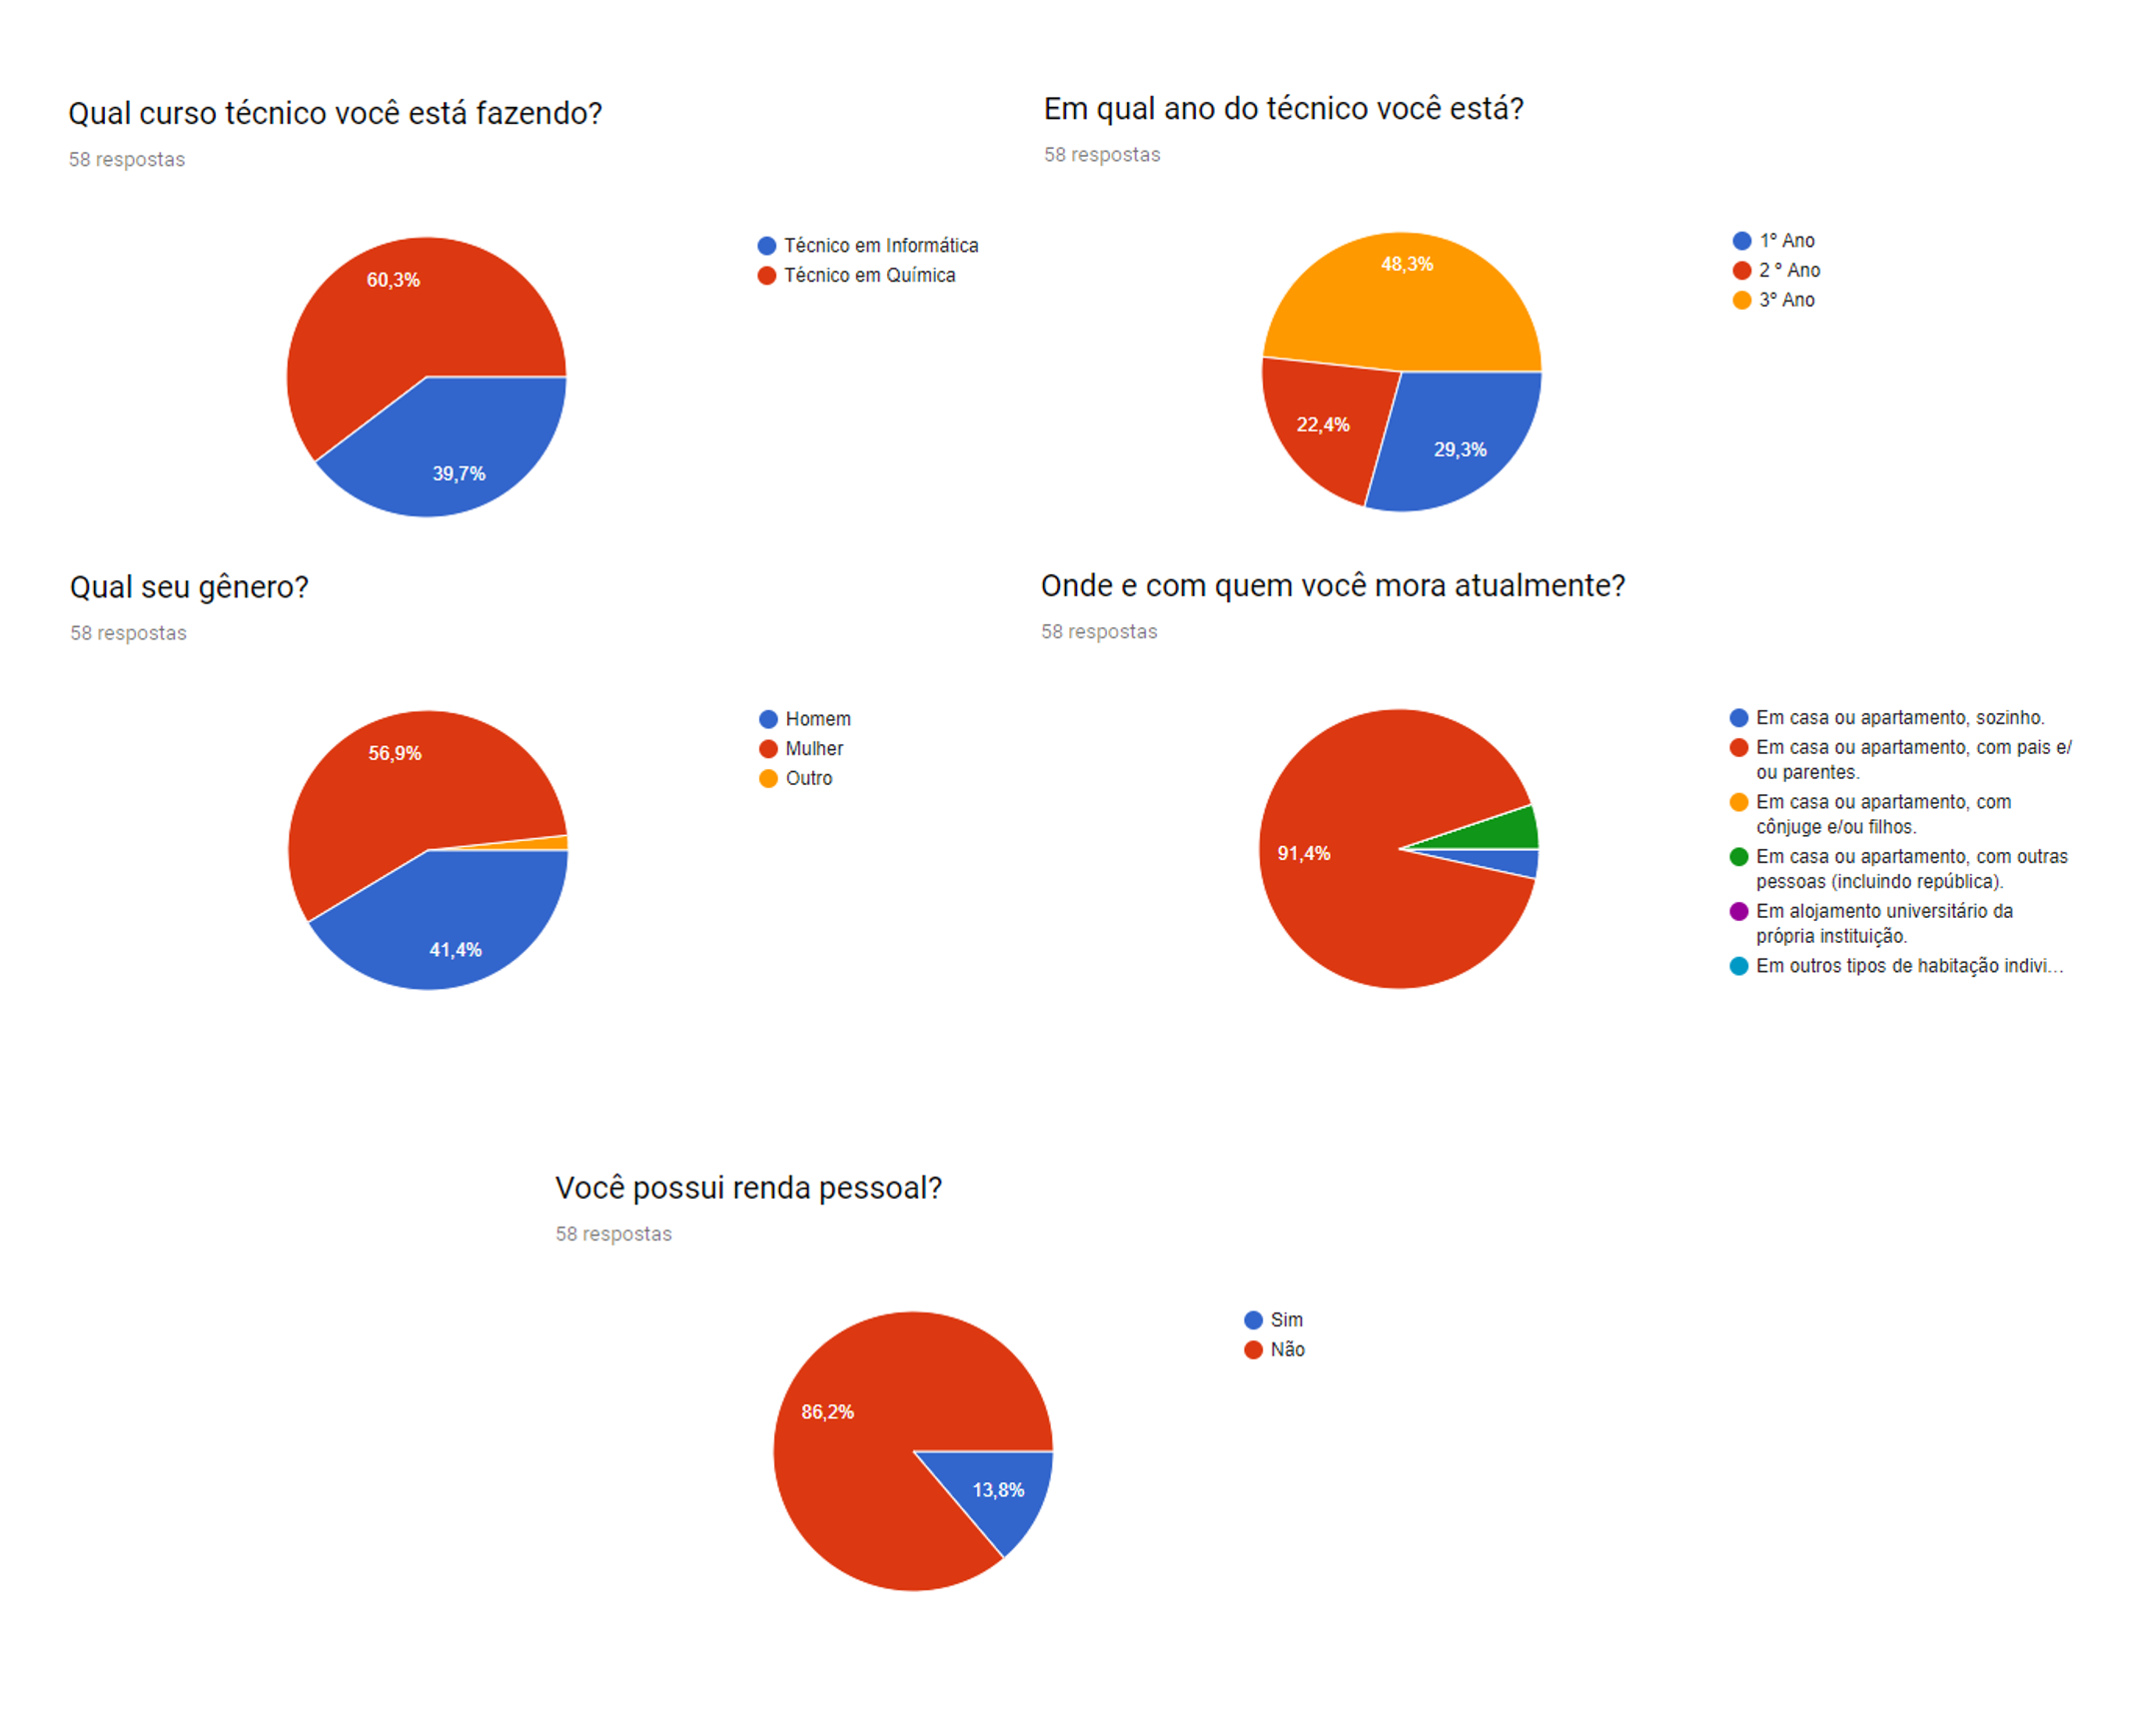
\includegraphics[width=1.0\textwidth]{img/quest1-5.png}
    \caption{Perguntas n$^{\underline{\circ}}$ 1 a 5}
    \label{fig:quest1-5}
\end{figure}

\begin{figure}[!htb]
    \centering
    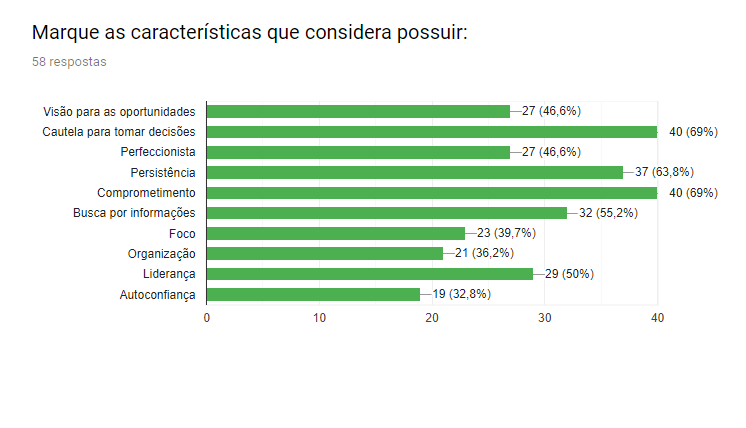
\includegraphics[width=0.9\textwidth]{img/habilidades.PNG}
    \caption{Características que os alunos acreditam possuir.}
    \label{fig:caract}
\end{figure}

\begin{figure}[!htb]
    \centering
    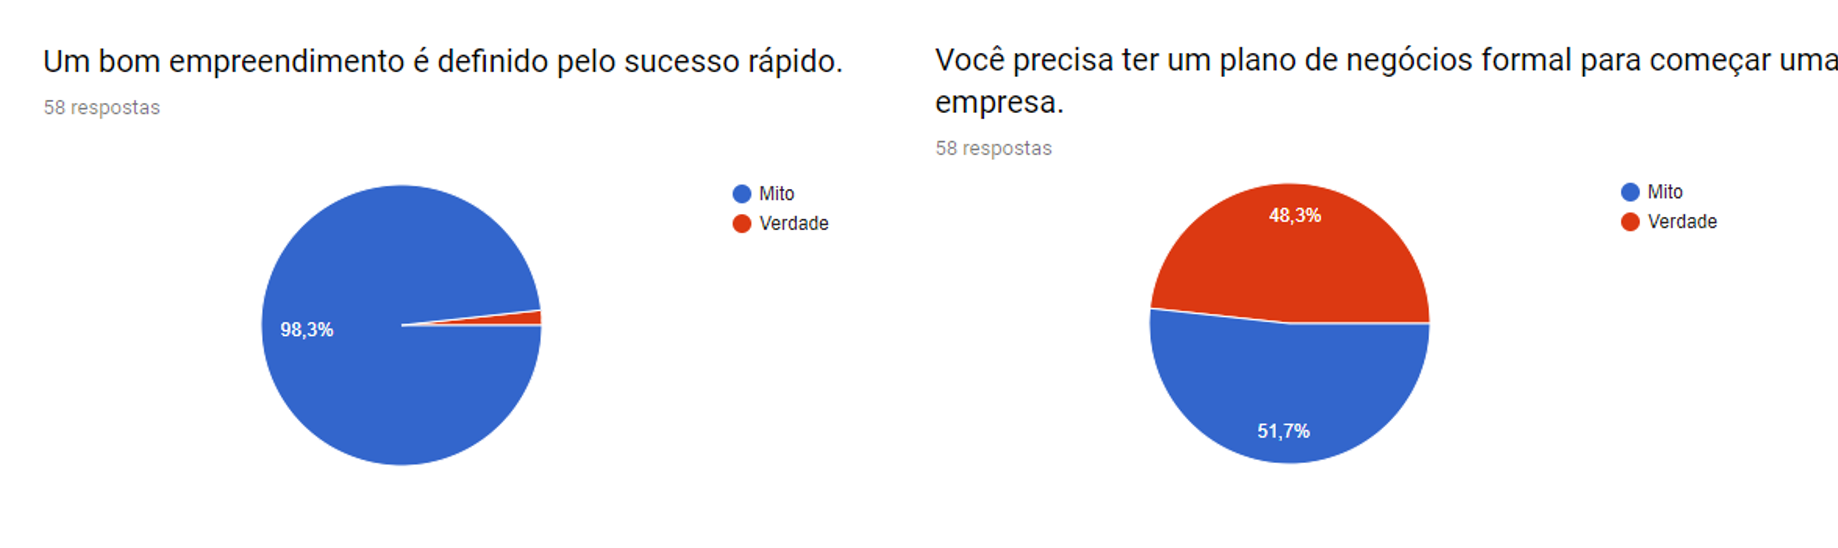
\includegraphics[width=1.0\textwidth]{img/mv1-2.png}
    \caption{$^{\underline{\circ}}$ Mitos e Verdades (a : Mito) e (b : Mito).}
    \label{fig:mv1-2}
\end{figure}

\begin{figure}[!htb]
    \centering
    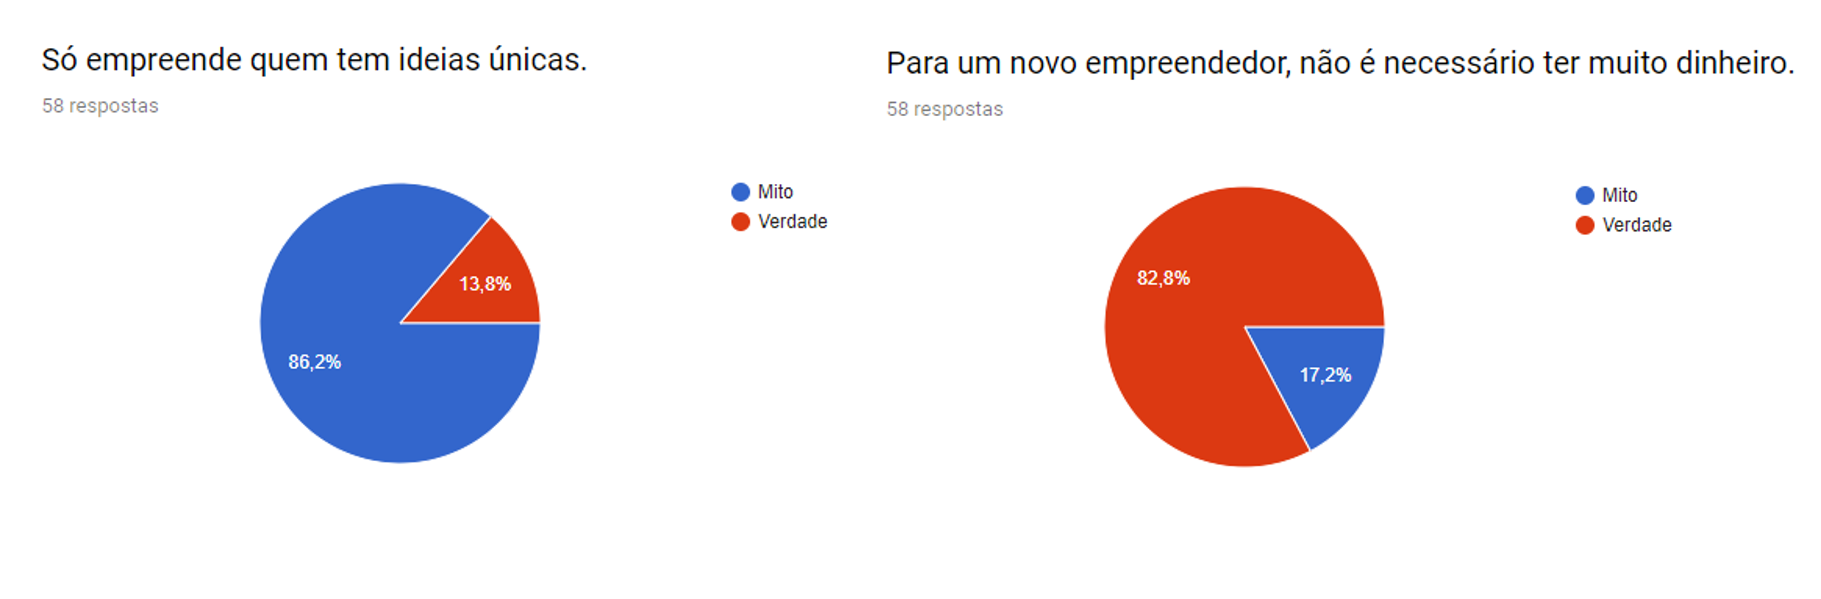
\includegraphics[width=1.0\textwidth]{img/mv3-4.png}
    \caption{$^{\underline{\circ}}$ Mitos e Verdades (c : Mito) e (d : Verdade).}
    \label{fig:mv3-4}
\end{figure}

\begin{figure}[!htb]
    \centering
    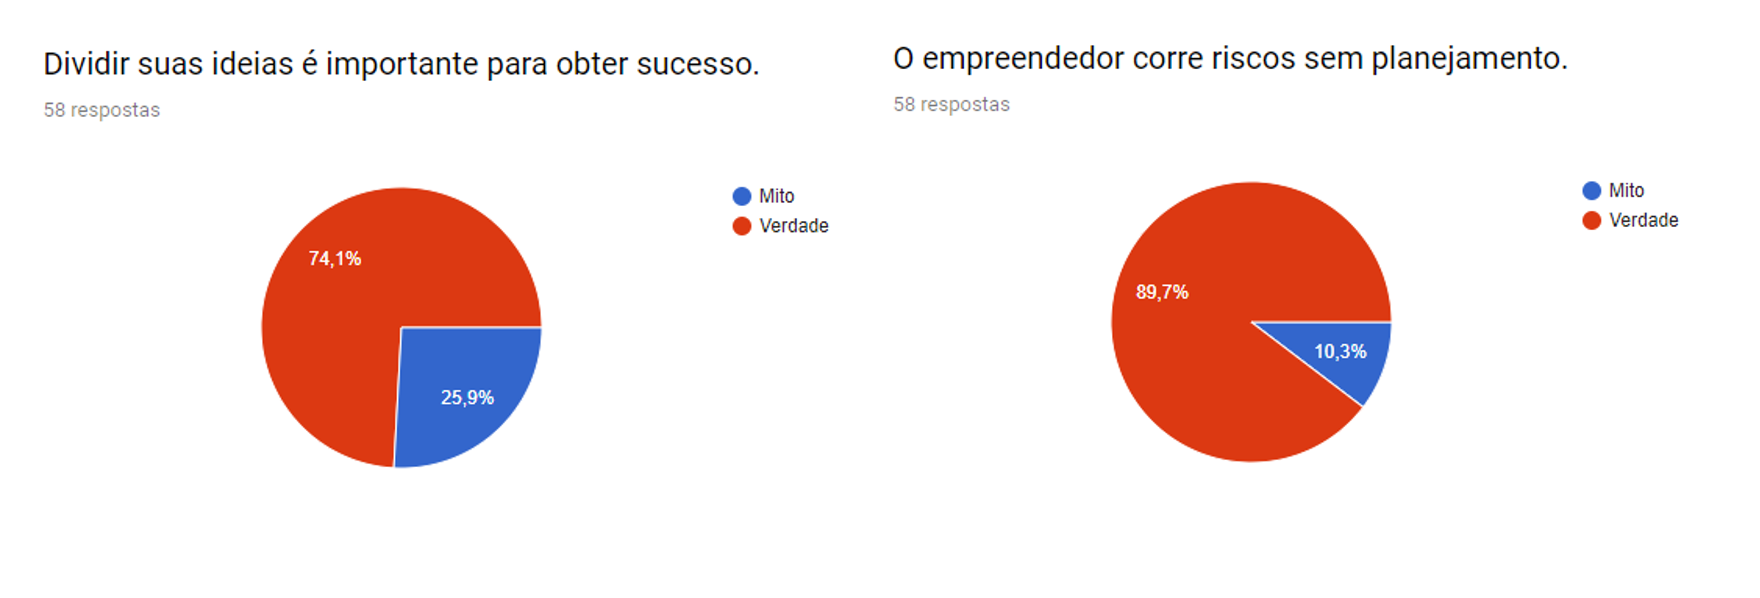
\includegraphics[width=1.0\textwidth]{img/mv5-6.png}
    \caption{$^{\underline{\circ}}$ Mitos e Verdades (e : Verdade) e (f : Mito).}
    \label{fig:mv5-6}
\end{figure}

